\documentclass{beamer}
\usepackage{ctex, hyperref}
\usepackage[T1]{fontenc}

% other packages
\usepackage{latexsym,amsmath,xcolor,multicol,booktabs,calligra}
\usepackage{graphicx,pstricks,listings,stackengine}
\usepackage{ruby,ulem,multirow}

\author{银河球棒侠}
\title{基于前端技术栈的\\ OpenStreetMap 中公共交通关系编辑器}
\subtitle{Frontend technology based OpenStreetMap PT relation editor}
\institute{OSMChina}
\date{2024年5月11日}
\usepackage{Tsinghua}

% defs
\def\cmd#1{\texttt{\color{red}\footnotesize $\backslash$#1}}
\def\env#1{\texttt{\color{blue}\footnotesize #1}}
\definecolor{deepblue}{rgb}{0,0,0.5}
\definecolor{deepred}{rgb}{0.6,0,0}
\definecolor{deepgreen}{rgb}{0,0.5,0}
\definecolor{halfgray}{gray}{0.55}

\lstset{
    basicstyle=\ttfamily\small,
    keywordstyle=\bfseries\color{deepblue},
    emphstyle=\ttfamily\color{deepred},    % Custom highlighting style
    stringstyle=\color{deepgreen},
    numbers=left,
    numberstyle=\small\color{halfgray},
    rulesepcolor=\color{red!20!green!20!blue!20},
    frame=shadowbox,
}


\begin{document}

\kaishu
\begin{frame}
    \titlepage
    \begin{figure}[htpb]
        \begin{center}
            
\includegraphics[width=0.2\linewidth]{figure/tuna.pdf}
        \end{center}
    \end{figure}
\end{frame}

\begin{frame}
    \tableofcontents[sectionstyle=show,subsectionstyle=show/shaded/hide,subsubsectionstyle=show/shaded/hide]
\end{frame}

\section{项目基础信息}

\begin{frame}
    \begin{itemize}
        \item 项目难度: 进阶 / Medium
        \item 项目社区导师:快乐的老鼠宝宝 / LaoshuBaby
        \item 导师联系方式:\href{mailto:me@jacksonzhao.email}{me@jacksonzhao.email}
    \end{itemize}
    \vspace{1.5em}
    $Ciallo\textasciitilde{}(\(\angle\cdot\omega<\))\textasciicircum{}\star$
\end{frame}

\subsection{项目描述}

\begin{frame}{高情商:具有较多技术债的现有项目}
    \quad \quad OpenStreetMap是英国人Steve Coast于2004年发起的以知识开放为原则的地图项目。\\
    \quad \quad 其数据模型对于公共交通等现实中抽象要素采用的关系描述方式较为复杂,OSM基金会从2016年至今每年都往GSOC提交公共交通相关的项目,但是成果和具有技术债的工具链关系密切,可用性不强。\\
    \quad \quad 本项目旨在以现代化的前端技术栈,实现一个可跨平台使用且操作简单交互明了的编辑器。\\
    \quad \quad 本项目过程中在交互和功能性上会与OSM中国社区合作。
\end{frame}

\begin{frame}
    \quad \quad OpenStreetMap is a map project initiated in 2004 by Steve Coast of the UK, based on the principle of knowledge openness. 
    Its data model employs a complex method of describing relationships for abstract elements in reality, such as public transport. \\
    \quad \quad Since 2016, the OSM Foundation has submitted projects related to public transport to GSOC annually, 
    but the outcomes are closely tied to a technically indebted toolchain, resulting in poor usability. \\
    \quad \quad This project aims to develop a cross-platform editor using a modern front-end technology stack, which is easy to use with clear interactions. \\
    \quad \quad During this project, there will be collaboration with the OSMChina community on interaction and functionality.
\end{frame}

\subsection{项目产出要求}

\begin{frame}
    \begin{enumerate}
        \item 能够在编辑器内添加站点并创建线路关系(关系内成员顺序可变)或删除关系并通过OSM API 0.6上传。
        \item 能在只有站点数据的情况下,根据图幅中路网和控制点自动计算可行的经由,和基于前述经由自动切割较长的路径以便于添加关系。
        \item 需实现至少包含主要功能的原型。
    \end{enumerate}
\end{frame}

\begin{frame}
    \begin{enumerate}
        \item Ability to add stations and create or delete route relationships (with variable member order) within the editor and upload them via OSM API 0.6.
        \item Ability to automatically calculate viable routes based on the road network and control points in the map, and automatically split longer paths for easier relationship addition, when only station data is available.
        \item Implementation of at least a prototype containing the main functionalities.
    \end{enumerate}
\end{frame}

\subsection{项目技术要求}

\begin{frame}
    \begin{enumerate}
        \item 能够使用前端技术栈开发具有复杂界面的跨平台程序,对WebGL有了解。(有用过Cesium.js/MapboxGL等WebGL的GIS框架属于加分项)
        \footnote{可能还需要一定的图形学和WASM知识\\(视最终技术栈选择而定。)}
        \item 有一定算法能力,对导航算法的实现有一定的了解。(有用过开源的导航路由工具如OSRM、Graphhopper、Valhalla等属于加分项。)
        \item 对OpenStreetMap的数据模型和API有所了解。(对社区文化和协作方式有了解或曾使用过相关数据进行分析等利用可视为加分项)
    \end{enumerate}
\end{frame}

\begin{frame}
    \begin{enumerate}
        \item Ability to use front-end technology stack to develop complex interface cross-platform programs, with knowledge of WebGL. (Experience with WebGL GIS frameworks such as Cesium.js/MapboxGL is a plus)
        \footnote{(Depending on the final choice of technology stack, knowledge of graphics and WASM might be required.)})
        \item Adequate algorithmic skills, with some understanding of navigation algorithm implementation. (Experience with open-source navigation routing tools like OSRM, Graphhopper, Valhalla, etc., is a plus.)
        \item Understanding of the OpenStreetMap data model and API. (Knowledge of community culture and collaboration methods, or previous use of related data for analysis or other purposes, is very important.)
    \end{enumerate}
\end{frame}


\subsection{相关的开源软件仓库列表}

\begin{frame}
    \begin{enumerate}
        \item \url{https://github.com/openstreetmap/iD} \\
        (关系编辑能力不强)
        \item \url{https://github.com/JOSM/pt_assistant} \\
        (不能独立于JOSM使用,较笨重)
        \item \url{https://github.com/Zaczero/osm-relatify} \\
        (一个偏实验性的编辑器原型,不适合大量编辑)
    \end{enumerate}
\end{frame}

\section{线路是如何被绘制的}

\begin{frame}
    \Large
    天天总是在各种地图看到公交线路,你有没有好奇过,它在地图上是用怎样的形式去存储的?
\end{frame}

\begin{frame}
	\begin{figure}[htpb]
		\centering
		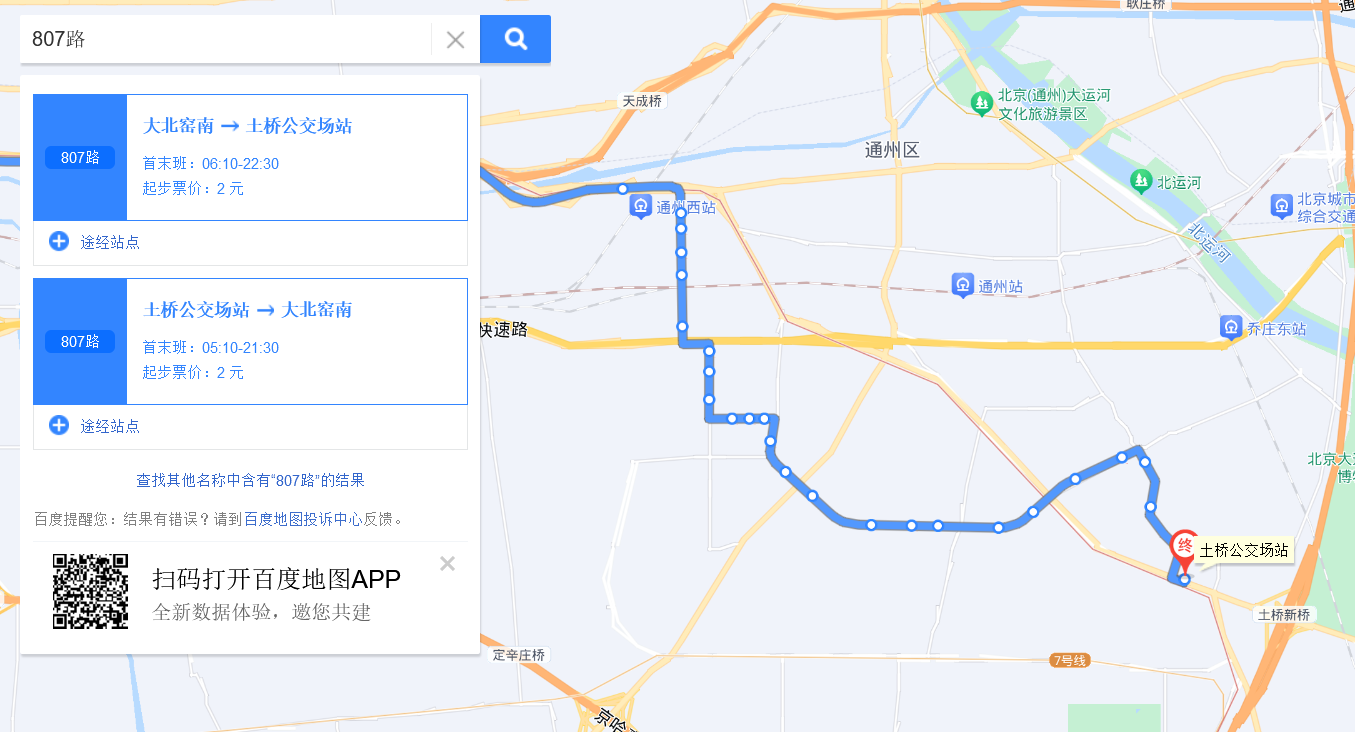
\includegraphics[width=1.15\linewidth]{figure/map_example-baidu-webbus.png}
	\end{figure}
\end{frame}

\begin{frame}
    \begin{columns}
        \column{0.5\textwidth}
        \begin{block}{}
            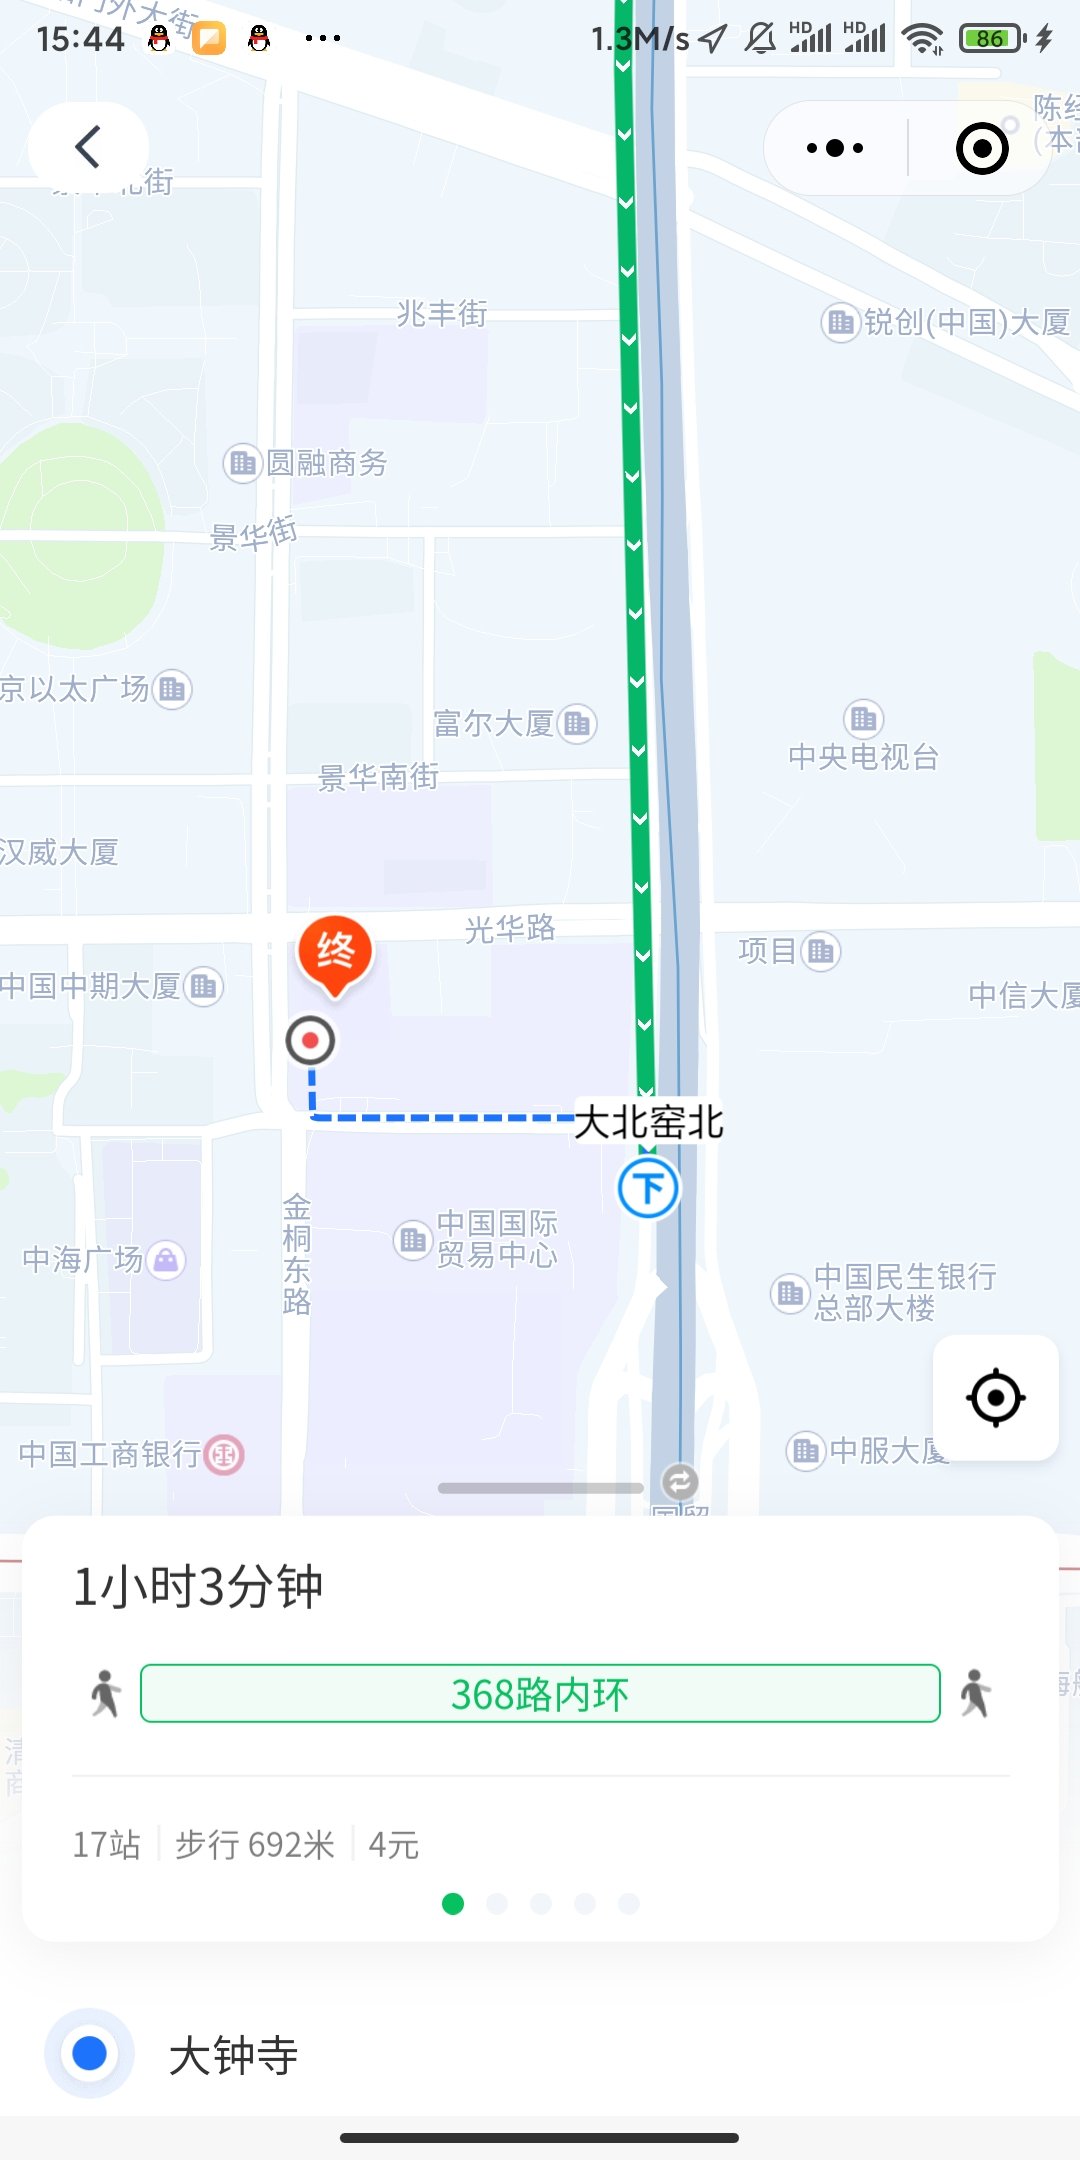
\includegraphics[width=0.7\linewidth]{figure/map_example-tencent-detail.jpg}
        \end{block}
        \column{0.5\textwidth}
        \begin{block}{}
            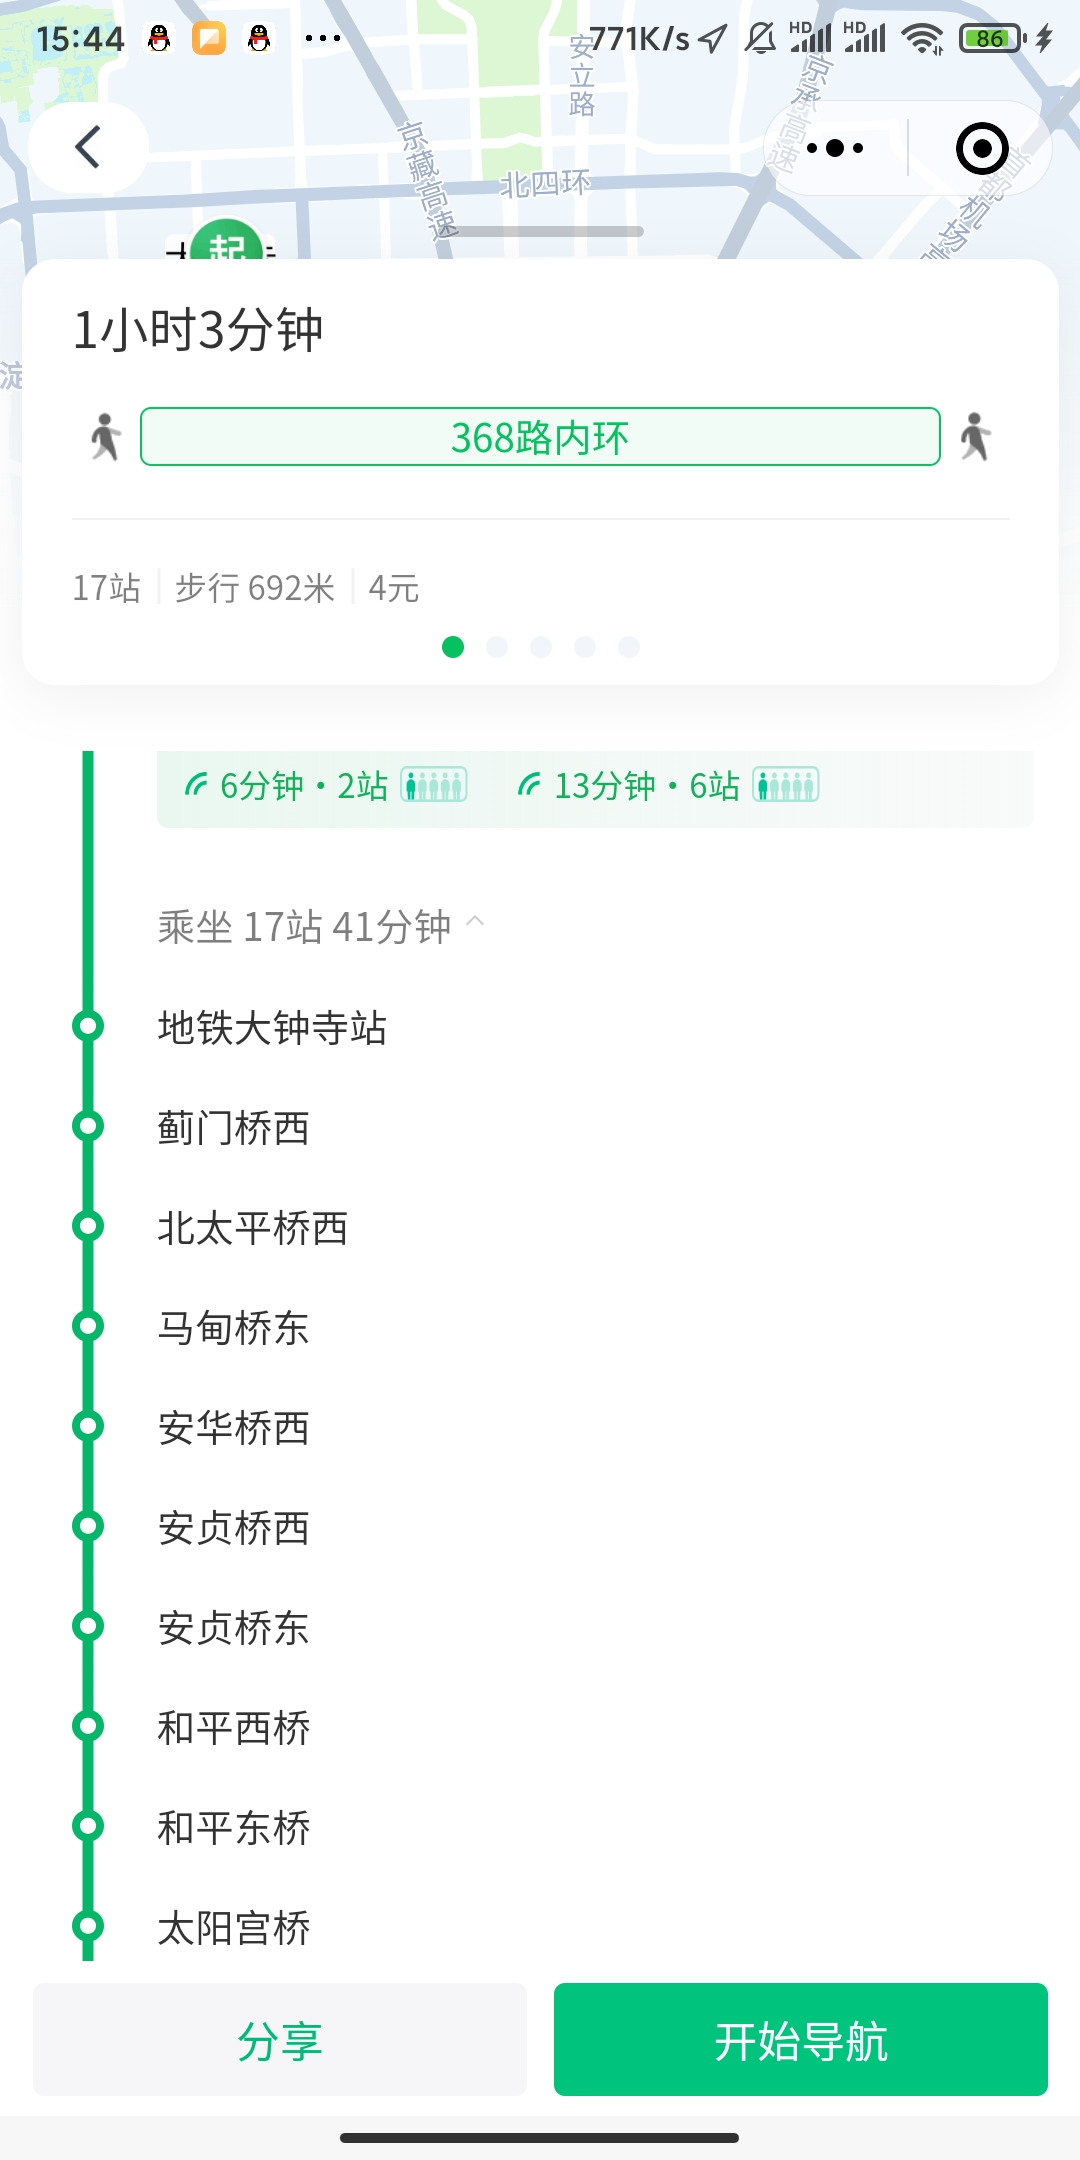
\includegraphics[width=0.7\linewidth]{figure/map_example-tencentbus.jpg}
        \end{block}
    \end{columns}
\end{frame}

\begin{frame}{现在的编辑器生态是怎样的}
    \Large
    \quad \quad 那如果我希望用OSM生态的编辑器去画一条公交线路呢?
\end{frame}

\begin{frame}{\sout{锐评}}
    \begin{figure}[htpb]
        \centering
        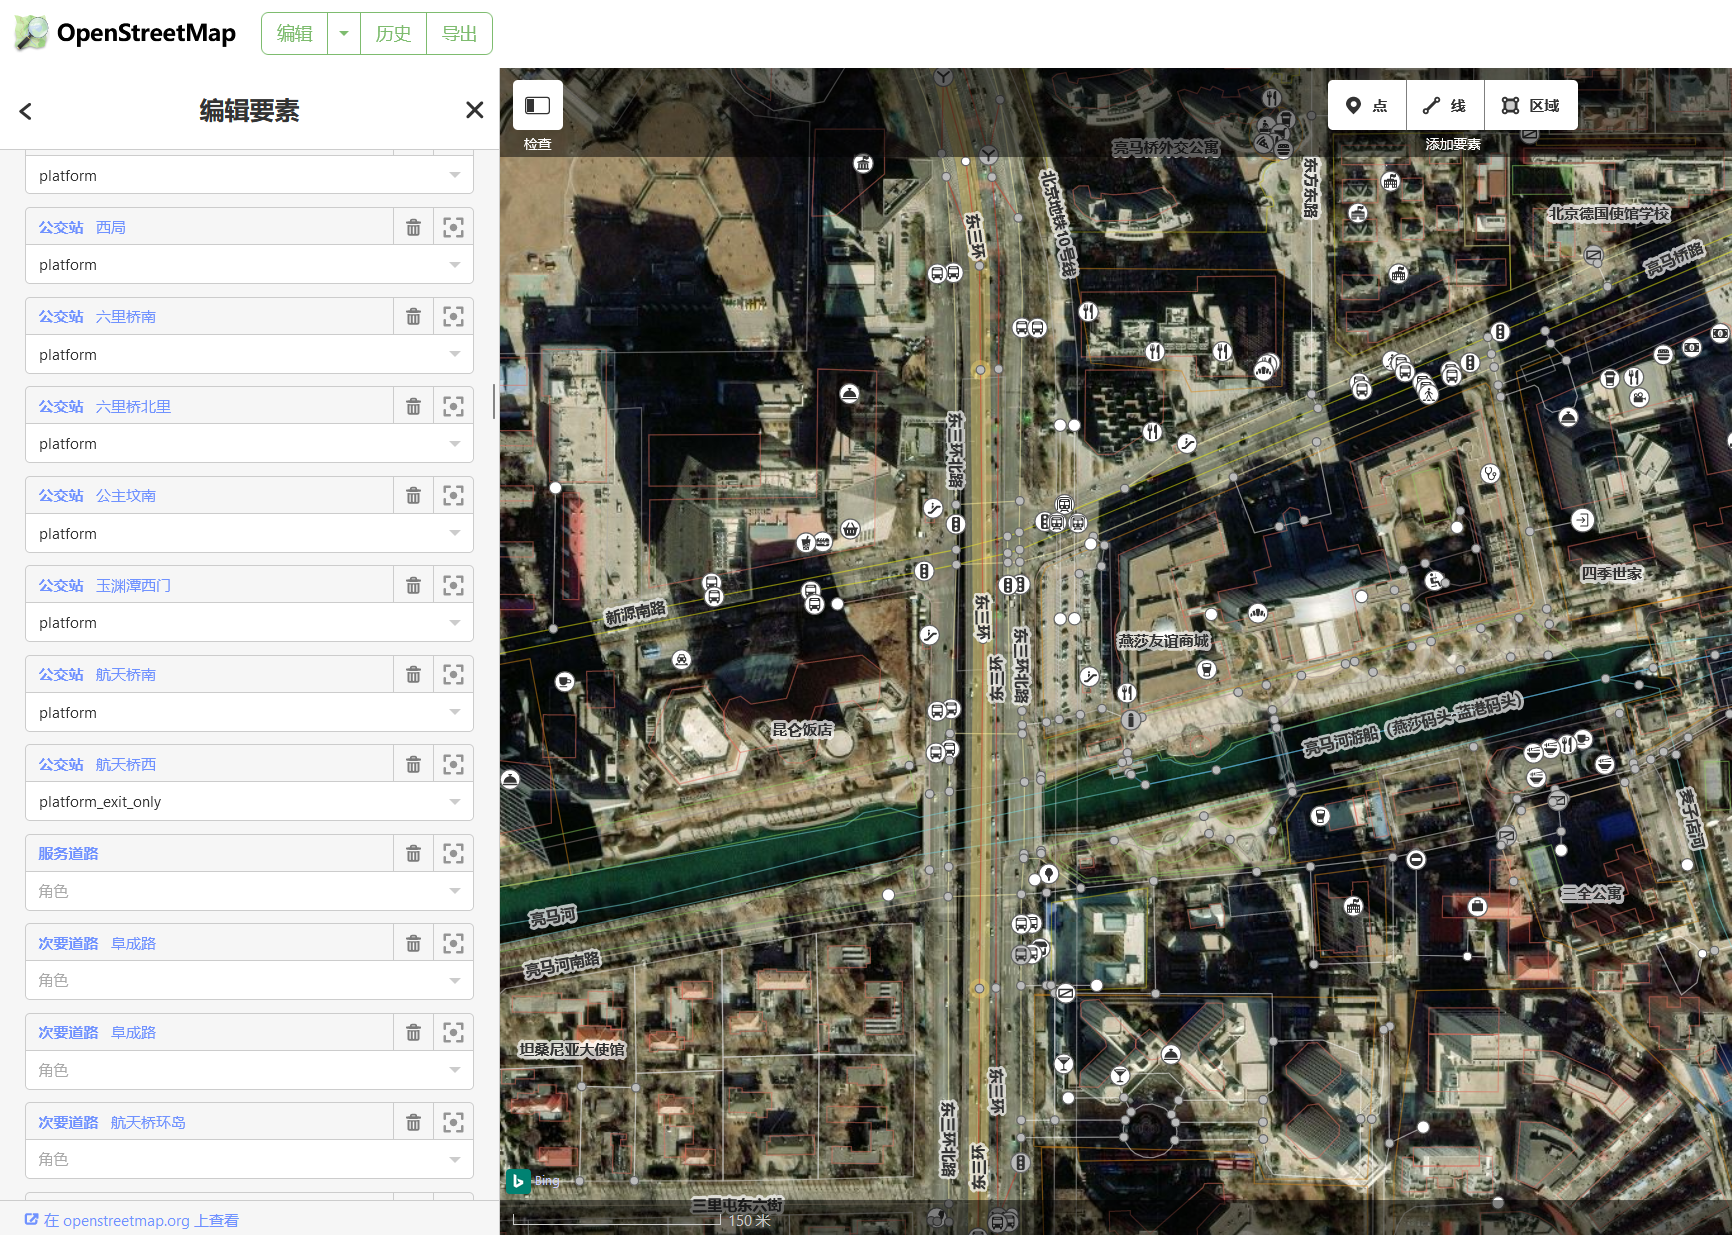
\includegraphics[width=0.75\linewidth]{figure/editor-iD.png}
        \caption{iD 编辑器中编辑公共交通线路的界面示例}
    \end{figure}
\end{frame}

\begin{frame}
    \quad \quad iD 编辑器是网页默认的编辑器,但是……
    \quad \quad 但是它调整起关系里面成员顺序的时候体验非常糟糕,你需要一个一个的拖拽上去,然后这个列表挪动的非常缓慢,并且难以在一屏内简单的看清所有成员,也不便于快速跳转到其他成员。\\
    \quad \quad 更致命的是,iD 编辑器内同时只能选中一个元素(Element,可以是Node、Way、Relation),你选择了成员的时候就会放弃对关系的选择,必须层层迭代去选中一个关系而难以稳定的直接选中。它默认不会提供一个索引。
    \quad \quad JOSM 编辑器是一个历史悠久的编辑器(甚至可能比在座一些同学的年龄都大)\\
    \quad \quad 但是功能确实繁琐,操作体验也不是很好,插件打多了就能体验到Java的图形性能了。
\end{frame}

\begin{frame}{\sout{锐评}}
    \begin{figure}[htpb]
        \centering
        \includegraphics[width=0.8\linewidth]{figure/editor-JOSM.png}
        \caption{JOSM 中编辑公共交通线路的界面示例}
    \end{figure}
\end{frame}

\begin{frame}
    \Large
    所以实际上绘制线路的流程是啥样的?
\end{frame}


\begin{frame}
    \begin{figure}[htpb]
        \centering
        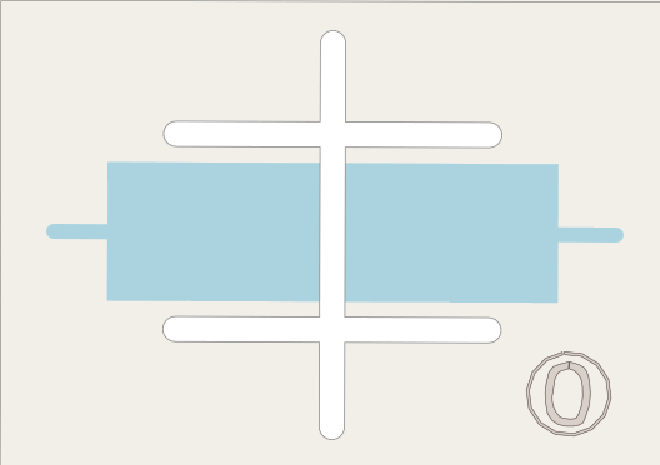
\includegraphics[width=1\linewidth]{figure/plot0.png}
    \end{figure}
\end{frame}

\begin{frame}
    \begin{figure}[htpb]
        \centering
        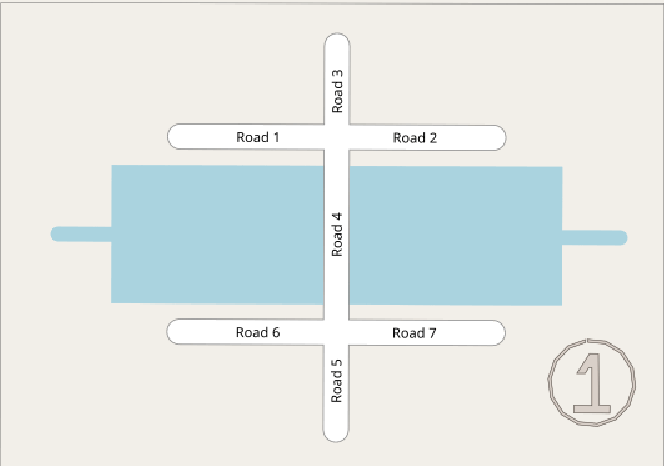
\includegraphics[width=1\linewidth]{figure/plot1.png}
    \end{figure}
\end{frame}

\begin{frame}
    \begin{figure}[htpb]
        \centering
        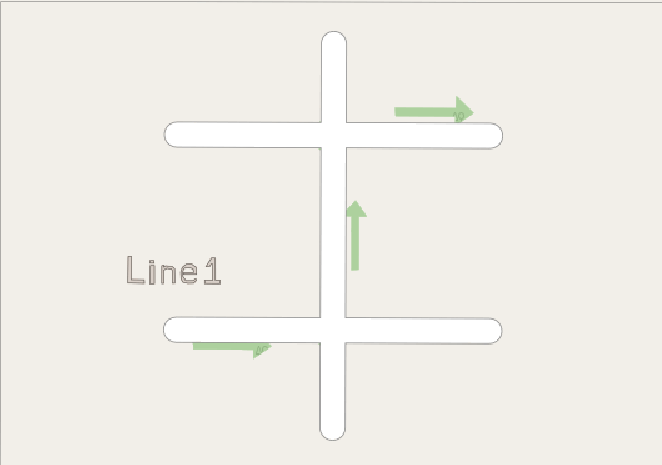
\includegraphics[width=1\linewidth]{figure/line1.png}
    \end{figure}
\end{frame}

\begin{frame}
    \begin{figure}[htpb]
        \centering
        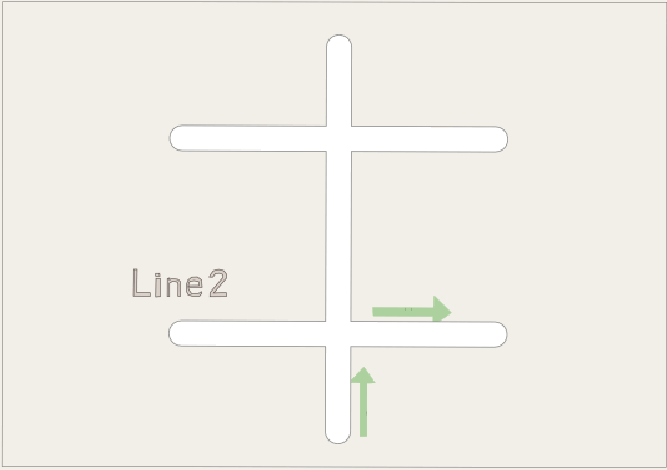
\includegraphics[width=1\linewidth]{figure/line2.png}
    \end{figure}
\end{frame}

\begin{frame}
    \begin{figure}[htpb]
        \centering
        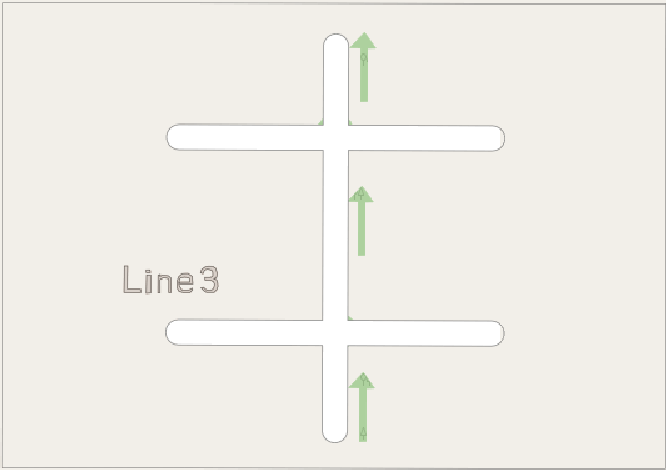
\includegraphics[width=1\linewidth]{figure/line3.png}
    \end{figure}
\end{frame}

\begin{frame}
    \begin{figure}[htpb]
        \centering
        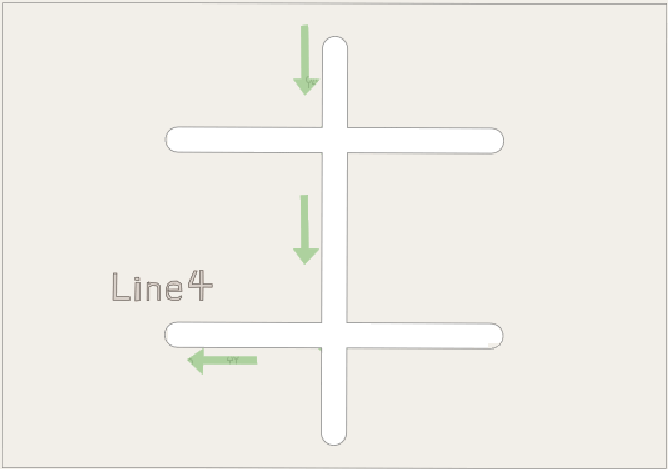
\includegraphics[width=1\linewidth]{figure/line4.png}
    \end{figure}
\end{frame}

\begin{frame}
    \begin{figure}[htpb]
        \centering
        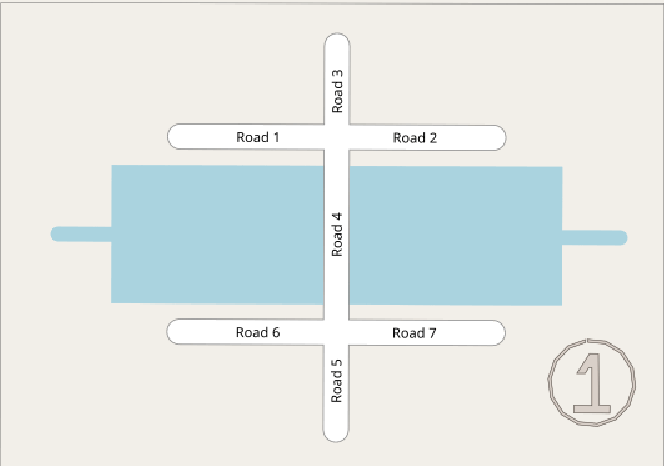
\includegraphics[width=0.95\linewidth]{figure/plot1.png}
    \end{figure}
    {
        \centering
        \quad \quad \quad \quad 现在回过头来再看这张图
    }
\end{frame}

\begin{frame}
    \begin{figure}[htpb]
        \centering
        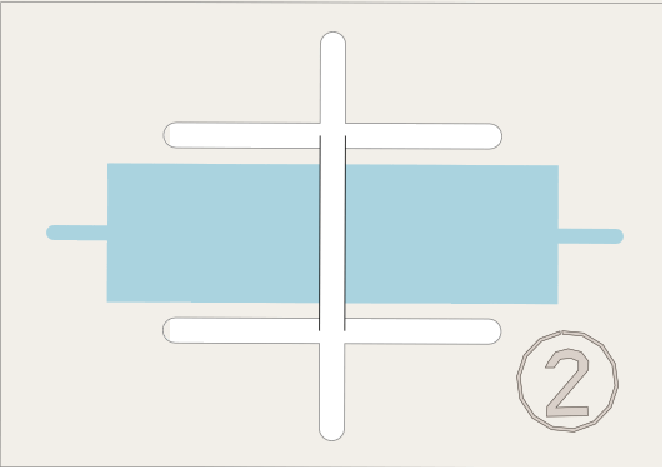
\includegraphics[width=1\linewidth]{figure/plot2.png}
    \end{figure}
\end{frame}

\begin{frame}
    \begin{figure}[htpb]
        \centering
        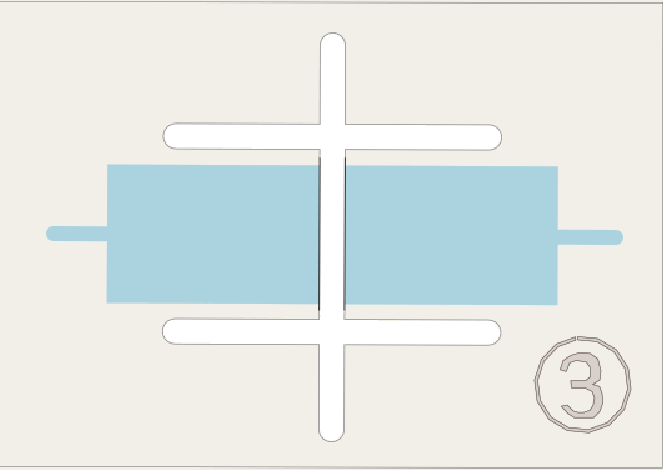
\includegraphics[width=1\linewidth]{figure/plot3.png}
    \end{figure}
\end{frame}

\section{或许需要剖析一下需要怎么做}

\begin{frame}
    前端技术方面的讨论,我建议去看看RapiD的那个演讲吧。\\
    Youtube有自动字幕,我也提供一个vtt对照翻译。英语好的同学想练习一下听力也是没问题的。 \\
    

    \begin{figure}[H]
        \centering
        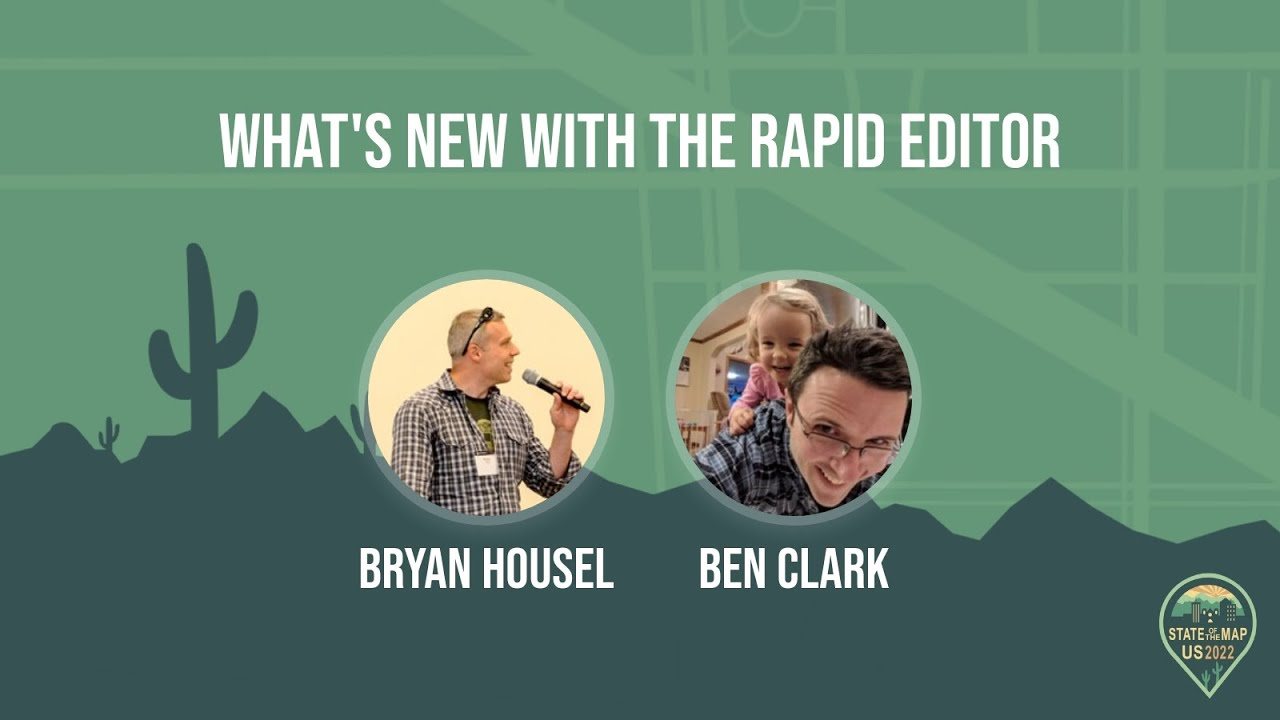
\includegraphics[width=0.7\textwidth]{figure/youtube-Kn7qusvEynU.jpg}
        \caption{What's new with the RapiD Editor - Bryan Housel \& Ben Clark}
    \end{figure}

    \url{https://m.youtube.com/watch?v=Kn7qusvEynU}
\end{frame}

\section{吐槽和\sout{梦中不可能之事}}

\begin{frame}
    \Large
    \sout{我一个后端佬,怎么就来带前端项目了呢?}\\
    \sout{所以说一个人的定位,不仅要看,也要……}
\end{frame}

\begin{frame}
    \large
    \quad \quad 首先我们知道,这个项目肯定会是一个持久的工程,不可能在本次OSPP期间全部完成。\\
    \vspace{4em}
    \quad \quad \textbf{“就一个编辑器就工作量这么大的吗?”}
\end{frame}


\begin{frame}
    \Large
    从公共交通的角度考虑:\\
    \normalsize
    \begin{itemize}
        \item 界面看起来比较粗糙怎么针对具体的绘图场景打磨?\\
        要不要印入小地图或者内嵌播放器可以同屏展示参考资料和街景?
        \item  有没有考虑过公交大小交路的混跑问题,它们都会混合在同一个主线关系下,如何识别?
        \item 部分地区的公交线路有局部自重叠的回环,能否正确处理?(举例:北京公交368路内环)
        \item 不同国家或地区公交网络结构不同,可能会和地铁混合在一起,如何准确识别?
    \end{itemize}
    
\end{frame}

\begin{frame}
    \Large
    从技术和应用开发的角度考虑: \\
    \normalsize
    \begin{itemize}
        \item 要不要把图面内的内容和具体地理坐标结合起来可编辑可拖拽?要不要印入id-tagging-schema的预设?
        \item 我们的编辑器不可能仅面向国内用户,如何按照用户喜欢的语言和文字进行本地化?
        \item OSM内的标签语义和显示文字以及使用的locale之间做好fallback和字形转换(CJK的“门”字、zh-CN和zh-Hans)
        \item 我们的编辑器在不同平台上可能有不同的交互逻辑,使用平板或其他触屏设备是否方便、使用移动设备能做出多少修改?\\
              不同浏览器下兼容性如何?
    \end{itemize}
\end{frame}

\begin{frame}
    \Large
    好,看起来头已经开始大了吧 \\
    \large
    \quad \quad 所以放宽心的,我们只需要实现最基本的公交路线关系编辑就可以 \\
    \quad \quad 很多功能都可以砍,都可以讨价还价(笑)\\
    \quad \quad 主要在于你有没有\textbf{想上手搞出这样一个工具的勇气}
\end{frame}

\section{计划进度}
\begin{frame}
    \quad \quad 一共就七月到九月,时间还是很紧张的,感觉上是真的做不完吧(笑) \\
    
    \quad \quad 所以如果想参赛,强烈建议描述你印象中最少的功能会主要由什么构成,并且尽量优先去实现。\\

    \quad \quad 另一个限制因素是我在五月下旬和整个六月都会非常忙
    \sout{(零分,下一个!负分,滚出去!)}\\

    \quad \quad 当然等开工以后,我会尽量做到每周和你\ruby{探讨进度}{\footnotesize Push \& PUA}一次甚至两次的 UwU!
\end{frame}

\begin{frame}
    \begin{center}
        {\Huge\calligra Thanks!}
    \end{center}
\end{frame}

\end{document}